\documentclass[UTF8,12pt]{article}
\usepackage{ctex}
\usepackage{indentfirst}
\usepackage{color}
\usepackage{hyperref}
\usepackage{graphicx}
\usepackage{subfigure}
\usepackage{pdfpages}
\usepackage{listings}
\usepackage{afterpage}
\usepackage{geometry}
\usepackage{booktabs}
\usepackage{multirow}
\usepackage{graphicx}

\geometry{a4paper,scale=0.8}

\newcommand\myemptypage{
    \null
    \thispagestyle{empty}
    \addtocounter{page}{-1}
    \newpage
}

\hypersetup{
    hidelinks,
	colorlinks=true,
	allcolors=black,
	pdfstartview=Fit,
	breaklinks=true
}

\definecolor{dkgreen}{rgb}{0,0.6,0}
\definecolor{gray}{rgb}{0.5,0.5,0.5}
\definecolor{mauve}{rgb}{0.58,0,0.82}

\lstset{ %
  language=Octave,                % the language of the code
  basicstyle=\footnotesize,           % the size of the fonts that are used for the code
  numbers=left,                   % where to put the line-numbers
  numberstyle=\tiny\color{gray},  % the style that is used for the line-numbers
  stepnumber=2,                   % the step between two line-numbers. If it's 1, each line 
                                  % will be numbered
  numbersep=5pt,                  % how far the line-numbers are from the code
  backgroundcolor=\color{white},      % choose the background color. You must add \usepackage{color}
  showspaces=false,               % show spaces adding particular underscores
  showstringspaces=false,         % underline spaces within strings
  showtabs=false,                 % show tabs within strings adding particular underscores
  frame=single,                   % adds a frame around the code
  rulecolor=\color{black},        % if not set, the frame-color may be changed on line-breaks within not-black text (e.g. commens (green here))
  tabsize=2,                      % sets default tabsize to 2 spaces
  captionpos=b,                   % sets the caption-position to bottom
  breaklines=true,                % sets automatic line breaking
  breakatwhitespace=false,        % sets if automatic breaks should only happen at whitespace
  title=\lstname,                   % show the filename of files included with \lstinputlisting;
                                  % also try caption instead of title
  keywordstyle=\color{blue},          % keyword style
  commentstyle=\color{dkgreen},       % comment style
  stringstyle=\color{mauve},         % string literal style
  escapeinside={\%*}{*)},            % if you want to add LaTeX within your code
  morekeywords={*,...}               % if you want to add more keywords to the set
}


\setlength{\parindent}{2em}

\begin{document}

\begin{titlepage}
    \includepdf[pages={1}]{cover1.pdf}
\end{titlepage}

\myemptypage

\begin{center}
    \tableofcontents
\end{center}

\newpage

% \section{实验1《GPIO端口实验》}

实验学时:2

每组人数:3

实验类别:2\ (1:基础性\ 2:综合性\ 3:设计性\ 4:研究性)

实验要求:1\ (1:必修\ 2:选修\ 3:其它)

实验类别:3\ (1:基础\ 2:专业基础\ 3:专业\ 4:其它)

\section{实验目的}
\begin{enumerate}
    \item 熟悉并掌握Keil MDK开发环境的使用以及在线调试方法;
    \item 掌握STM32F746NG芯片GPIO端口寄存器的配置;
    \item 通过实验掌握Cortex-M7控制GPIO端口的方法,实现对LED的控制。
\end{enumerate}

\section{实验内容}
编写程序,对指定GPIO端口进行初始化并完成配置过程,实现对LED的控制。学习使用超级终端,对其进行配置并完成串口调试。实验中观察GPIO端口输出数据寄存器(GPIOx\_ODR)的值对LED灯的明灭的影响,学习GPIO端口的输入输出方式、输出类型和输出速度的设置方法。

\section{实验方法}

\subsection{实验原理}
STM32F746NG芯片共有168个GPIO(通用I/O)端口(GPIOA~GPIOK),每个GPIO端口均可以通过软件配置为输出、输入或复用功能。

\begin{enumerate}
    \item GPIO主要特性
    \begin{itemize}
        \item 输出状态:推挽或开漏+上拉/下拉;
        \item 从输出数据寄存器(GPIOx\_ODR)或外设(复用功能输出)输出数据;
        \item 可为每个I/O选择不同的速度;
        \item 输入状态:浮空、上拉/下拉、模拟;
        \item 将数据输入到输入数据寄存器(GPIOx\_ODR)或外设(复用功能输入);
        \item 置位和复位寄存器(GPIOx\_BSRR),对GPIOx\_ODR具有按位写权限;
        \item 锁定机制(GPIOx\_LCKR),可冻结I/O端口配置;
        \item 模拟功能;
        \item 复用功能选择寄存器;
        \item 快速翻转,每次翻转最快只需要两个时钟周期;
        \item 引脚复用非常灵活,允许将I/O引脚用作GPIO或多种外设功能中的一种。
    \end{itemize}
    \item GPIO功能描述

    每个GPIO端口的各个端口位均可以自由编程,通过对相关寄存器的修改可以配置为多种模式:
    \begin{itemize}
        \item 浮空输入
        \item 上拉输入
        \item 下拉输入
        \item 模拟输入/输出
        \item 具有上拉或下拉功能的开漏输出
        \item 具有上拉或下拉功能的推挽输出
        \item 具有上拉或下拉功能的复用功能推挽
        \item 具有上拉或下拉功能的复用功能开漏
    \end{itemize}
    对I/O端口进行编程作为输入时,输出缓冲器被禁止,施密特触发器输入被打开,根据GPIOx\_PUPDR寄存器中的值决定是否打开上拉和下拉电阻,输入数据寄存器每隔1个AHB时钟周期对I/O引脚上的数据进行一次采样,对输入数据寄存器的读访问可获取I/O状态。

    对I/O端口进行编程作为输出时,输出缓冲器被打开,施密特触发器输入被打开,根据GPIOx\_PUPDR寄存器中的值决定是否打开上拉和下拉电阻,输入数据寄存器每隔1个AHB时钟周期对I/O引脚上的数据进行一次采样,对输入数据寄存器的读访问可获取I/O状态,对输出数据寄存器的读访问可获取最后的写入值。

    对I/O端口进行编程作为复用功能时,可将输出缓冲器配置为开漏或推挽模式,输出缓冲器由来自外设的信号驱动,施密特触发器输入被打开,根据GPIOx\_PUPDR寄存器中的值决定是否打开上拉和下拉电阻,输入数据寄存器每隔1个AHB时钟周期对I/O引脚上的数据进行一次采样,对输入数据寄存器的读访问可获取I/O状态。

    对I/O端口进行编程作为模拟配置时,输出缓冲器被禁止,施密特触发器输入停用,I/O引脚的每个模拟输入的功耗变为零,施密特触发器的输出被强制处理为恒定值(0),弱上拉和下拉电阻被硬件关闭,对输入数据寄存器的读访问值为“0”。

    \item GPIO寄存器

    每个通用I/O端口包括4个32位配置寄存器(GPIOx\_MODER、GPIOx\_OTYPER、GPIOx\_OSPEEDR 和 GPIOx\_PUPDR)、2个32位数据寄存器(GPIOx\_IDR 和 GPIOx\_ODR)和1个32位置位/复位寄存器 (GPIOx\_BSRR)。此外,所有GPIO都包括1个32位锁定寄存器 (GPIOx\_LCKR) 和2个32位复用功能选择寄存器(GPIOx\_AFRH 和 GPIOx\_AFRL)。I/O端口寄存器必须按32位字、半字或字节进行访问。
    \item GPIO寄存器边界地址
    
    STM43F746NG的GPIO寄存器边界地址如表所示
    \begin{table}[!ht]
        \centering
        \begin{tabular}{|l|l|}
        \hline
            外设 & 寄存器边界地址  \\ \hline
            GPIOA & 0x4002 0000 – 0x4002 03FF  \\ \hline
            GPIOB & 0x4002 0400 – 0x4002 07FF  \\ \hline
            GPIOC & 0x4002 0800 – 0x4002 0BFF  \\ \hline
            GPIOD & 0x4002 0C00 – 0x4002 0FFF  \\ \hline
            GPIOE & 0x4002 1000 – 0x4002 13FF  \\ \hline
            GPIOF & 0x4002 1400 – 0x4002 17FF  \\ \hline
            GPIOG & 0x4002 1800 – 0x4002 1BFF  \\ \hline
            GPIOH & 0x4002 1C00 – 0x4002 1FFF  \\ \hline
            GPIOI & 0x4002 2000 – 0x4002 23FF  \\ \hline
        \end{tabular}
    \end{table}

    \item 实验电路
    
    实验电路如图所示

    \begin{figure}[htbp]
        \centering
        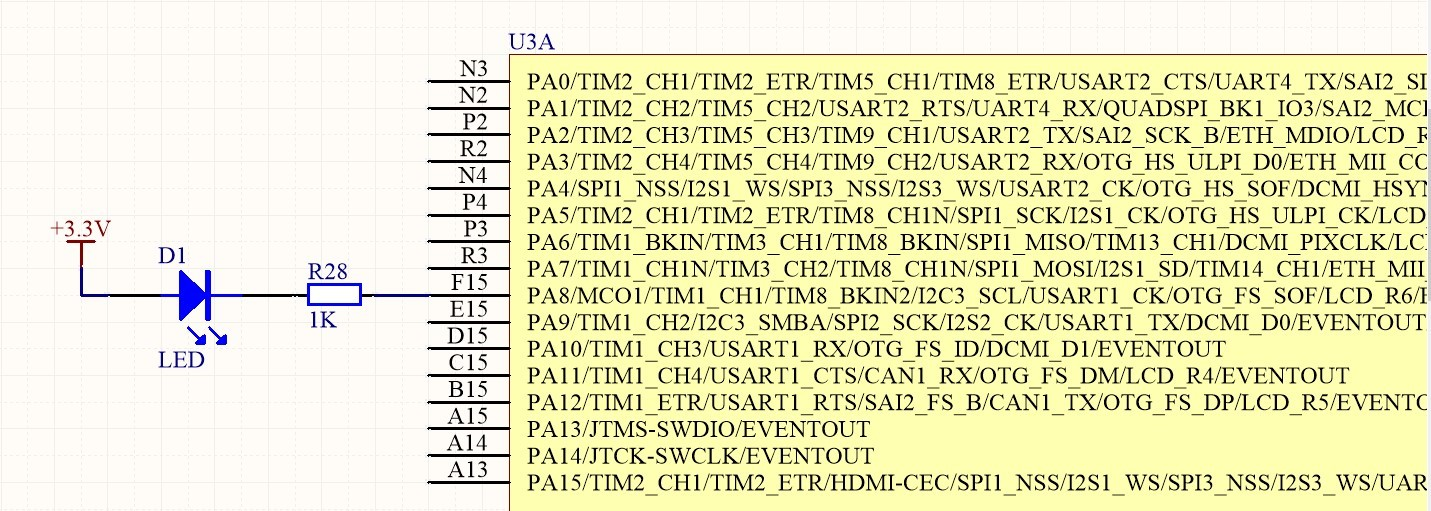
\includegraphics[width=0.8\textwidth]{imgs/1.jpg}
        \caption{实验电路}
    \end{figure}

    如图中所示,U3A单元为STM32F746芯片,发光二极管D1一端与VCC相连,另一端经过1K电阻与Cortex-M7的PA8(GPIOA8)相连,将PA8配置为输出I/O口,即可通过控制其高低电平状态进而控制发光二极管D1的的亮与灭。当PA8输出低电平时,电路导通,发光二极管D1点亮;反之,发光二极管D1熄灭。实验例程中,每次对PA8的输出状态取反后调用延时函数,使发光二极管保持亮或灭,循环往复即可实现发光二极管的闪烁。通过修改延时长度,可以改变发光二极管的闪烁频率。

\end{enumerate}

\subsection{实验方案及调试过程}
\noindent
\textbf{基础实验}:首先复现例程代码,得到指导书期望现象并记录
\noindent
实验例程如下:

\begin{lstlisting}[frame=shadowbox]
    /**
    主程序:系统上电初始化后对GPIO中的PA8进行配置,将其配置为输出端口并控制LED闪烁。
  **/
  #include "main.h"
  #include "system_init.h"
  
  /* Private variables */
  uint16_t delay = 100;
  
  void System_Init(void);
  void GPIO_Config(void);
  
  /* main */
  int main(void)
  {
    System_Init();
    
    GPIO_Config();
    
    printf("\n\rExample finished\n\r");
      
    /* Toggle IOs in an infinite loop */
    while (1)
    {
      HAL_GPIO_TogglePin(GPIOA, GPIO_PIN_8);
      /* Insert delay */
      HAL_Delay(delay);
    }
  }  
\end{lstlisting}
调试过程如下:

首先定义了私有变量delay,用于控制延时时间:uint16\_t delay = 100;

然后调用System\_Init()函数进行系统初始化,调用GPIO\_Config()函数对GPIO端口进行初始化。

\begin{lstlisting}[frame=shadowbox]
void System_Init(void)
{
  /* Enable the CPU Cache */
  CPU_CACHE_Enable();

  /* STM32F7xx HAL library initialization */
  HAL_Init();

  /* Configure the system clock to 216 MHz */
  SystemClock_Config();
  
  /* Configure UART */
  UART_Config();
  
  printf("\n\rSystem initialize success\n\r");
}
\end{lstlisting}
GPIO\_Config()函数的定义如下:

\begin{lstlisting}[frame=shadowbox]
void GPIO_Config(void)
{
/* Enable each GPIO Clock (to be able to program the configuration registers) */
  __HAL_RCC_GPIOA_CLK_ENABLE();
  
  /* Configure IOs in output push-pull mode to drive external LED */
  GPIO_InitStruct.Mode  = GPIO_MODE_OUTPUT_PP;	// 推挽输出
  GPIO_InitStruct.Pull  = GPIO_PULLUP;					// 上拉
  GPIO_InitStruct.Speed = GPIO_SPEED_HIGH;			// 高速

  GPIO_InitStruct.Pin = GPIO_PIN_8;
  HAL_GPIO_Init(GPIOA, &GPIO_InitStruct);				// 引脚为PA8
}

\end{lstlisting}
然后进入死循环状态,通过调用HAL\_GPIO\_TogglePin()函数对GPIOA的8号引脚进行翻转,即实现LED灯的闪烁效果。具体的实现如下:

\begin{lstlisting}[frame=shadowbox]
void HAL_GPIO_TogglePin(GPIO_TypeDef* GPIOx, uint16_t GPIO_Pin)
{
  /* Check the parameters */
  assert_param(IS_GPIO_PIN(GPIO_Pin));

  GPIOx->ODR ^= GPIO_Pin;
}
\end{lstlisting}
利用异或操作实现对GPIO引脚状态的翻转。

每次翻转后调用HAL\_Delay()函数进行延时,延时时间为delay,以控制LED灯的闪烁频率。具体实现如下:

\begin{lstlisting}[frame=shadowbox]
__weak void HAL_Delay(__IO uint32_t Delay)
{
  uint32_t tickstart = 0;
  tickstart = HAL_GetTick();
  while((HAL_GetTick() - tickstart) < Delay)
  {
  }
}
\end{lstlisting}
HAL\_Delay()函数通过调用HAL\_GetTick()函数获取当前的系统滴答计数值,然后通过循环判断当前的系统滴答计数值与tickstart的差值是否小于Delay,若小于则继续循环,否则退出循环,从而实现延时效果。

\noindent
\textbf{进阶实验}:请自行搜索摩尔斯密码表,通过控制D1的亮灭间隔,实现自己姓氏拼音的电码实现。

摩尔斯电码(Morse code)也被称作摩斯密码,是一种时通时断的信号代码,通过不同的排列顺序来表达不同的英文字母、数字和标点符号。这里我们通过控制D1的亮灭间隔,实现自己姓氏拼音的电码。

具体的算法思路如下:

\begin{enumerate}
    \item 姓氏的拼音用英文打出,姓氏拼音有多个英文字母组成,英文字母之间用空格隔开,每一个姓之间用逗号隔开;
    \item 定义短信号和长信号的时间分别为200ms和600ms,空格时长1000ms,逗号时长2000ms,正常信号之间的间隔为200ms;
\end{enumerate}

第一步中,我们小组有三位成员,分别姓:
% // wjy-WU=".-- ..-"
% // gx-GUO="--. ..- ---"
% // zzy-ZOU="--.. --- ..-"

\begin{itemize}
    \item WU=".-- ..-"
    \item GUO="--. ..- ---"
    \item ZOU="--.. --- ..-"
\end{itemize}

因此我们定义字符数组:
\begin{lstlisting}[frame=shadowbox]
char lname[]=".-- ..-,--. ..- ---,--.. --- ..-";
\end{lstlisting}

然后定义短信号和长信号的时间分别为200ms和600ms,空格时长1000ms,逗号时长2000ms,正常信号之间的间隔为200ms。

\begin{lstlisting}[frame=shadowbox]
uint16_t delay = 100;
uint16_t short_delay=200;
uint16_t long_delay=600;
uint16_t blank_delay=1000;
uint16_t gap_delay=2000;
\end{lstlisting}

根据电码序列的不同字母('.'/'-'/' '/',')分别使用短延迟、长延迟、空格延迟、逗号延迟的时长进行延迟,从而控制灯亮灭的间隔。

在死循环中,对整个字符数组进行遍历,根据字符的不同,进行不同的延迟操作,从而实现对LED灯的控制。

\begin{lstlisting}[frame=shadowbox]
    while(1){
        //turn on the LED light
        HAL_GPIO_TogglePin(GPIOA, GPIO_PIN_8);
        if(lname[i%31]=='.'){
          HAL_Delay(short_delay);
        }else if(lname[i%31]=='-'){
          HAL_Delay(long_delay);
        }
        //turan off the LED light
        HAL_GPIO_TogglePin(GPIOA, GPIO_PIN_8);
        //control delay of off state
        if(lname[(i+1)%31]==' '){
          HAL_Delay(blank_delay);
          i+=2;
        }
        else if(lname[(i+1)%31]==','){
          HAL_Delay(gap_delay);
          i+=2;
        }else{
          HAL_Delay(delay);
          i++;
        }
    }
\end{lstlisting}

\section{实验步骤}
\subsection{准备实验环境}
使用ULINK2 USB-JTAG仿真器连接ARM Cortex-M7实验板与PC,实验板一侧接P1接口。使用串口线,连接实验板上的串口J3和PC机的串口。接口P1和J3的位置如图所示。

\begin{figure}[htbp]
    \centering
    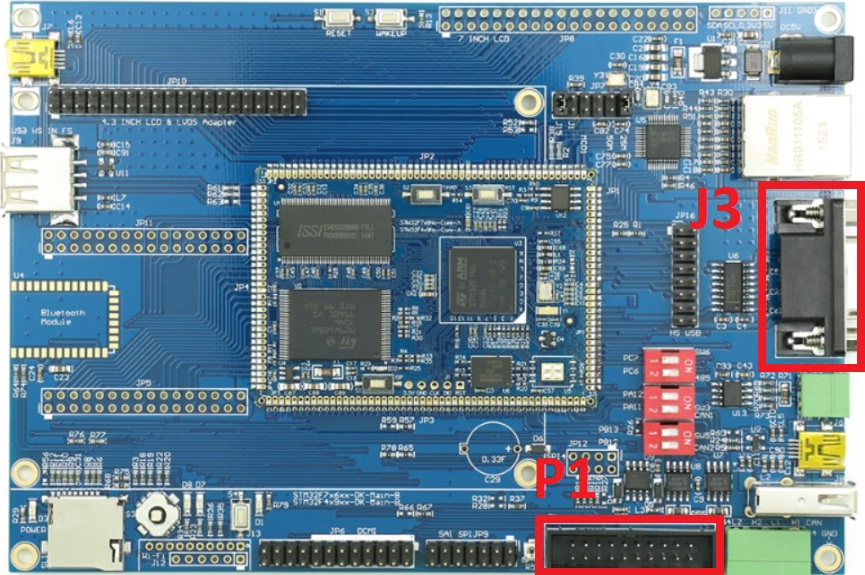
\includegraphics[width=0.8\textwidth]{imgs/2.png}
    \caption{接口P1和J3在实验板中的位置图}
\end{figure}

\subsection{串口接收设置}
在PC机上运行windows自带的超级终端串口通信程序(波特率115200 、1 位停止位、无校验位、无硬件流控制);或者使用其它串口通信程序。 

\subsection{打开实验例程}
拷贝实验平台附带程序“02\_GPIO”,使用$\mu$Vision IDE for ARM通过 ULINK2 USB-JTAG仿真器连接实验板,打开工程文件,编译链接工程,点击MDK的Project菜单,选择Rebuild all target files进行编译,编译成功后,点击Debug菜单,选择Start/Stop Debug Session项或点击工具栏中的 图标,下载工程生成的.axf 文件到目标板的 RAM中调试运行。

\subsection{观察实验结果}
结合实验内容和相关资料,使用一些调试命令,观察程序运行。注意观察发光二极管的亮灭情况,观察到的现象与前面实验内容中的相符,则说明实验程序通过配置GPIO引脚的输出状态实现了对发光二极管的控制。修改代码,实现自己姓氏的摩尔斯电码。


\section{实验结果}


\section{实验结论}
本实验中,我们通过HAL\_GPIO\_TogglePin()可以切换LED灯状态,利用异或(XOR)操作取反GPIOx对应位的值,达到反转指定引脚状态的效果;同时,我们可以通过控制HAL\_GPIO\_TogglePin()的间隔来控制亮灯和灭灯的时间,对不同的字符设置不同的间隔时间来实现自己姓氏拼音的电码。实验源代码见附录。

\section{实验小结}
通过本实验,我更加熟练地掌握了vscode+Keil MDK开发环境的使用以及在线调试方法,对STM32F746NG芯片GPIO端口寄存器的配置有了更加直观的认识,并对C语言嵌入式编程有了初步的认识,收获很大。

\newpage

\section{实验1源代码}
\begin{lstlisting}[frame=shadowbox]
    /**
    主程序:系统上电初始化后对GPIO中的PA8进行配置,将其配置为输出端口并控制LED闪烁。
  **/
  #include "main.h"
  #include "system_init.h"
  
  /* Private variables */
  uint16_t delay = 100;
  
  uint16_t short_delay=200;
  uint16_t long_delay=600;
  uint16_t blank_delay=1000;
  uint16_t gap_delay=2000;
  
  void System_Init(void);
  void GPIO_Config(void);
  
  /* main */
  int main(void)
  {
    System_Init();
    
    GPIO_Config();
    
    printf("\n\rExample finished\n\r");
  
    // wjy-WU=".-- ..-"
    // gx-GUO="--. ..- ---"
    // zzy-ZOU="--.. --- ..-"
    char lname[]=".-- ..-,--. ..- ---,--.. --- ..-";
    int i=0;
  
    /* Toggle IOs in an infinite loop */
    // while (1)
    // {
    //   HAL_GPIO_TogglePin(GPIOA, GPIO_PIN_8);
    //   /* Insert delay */
    //   HAL_Delay(delay);
    // }
  
    // 打印姓氏
    // 方法:
    // 形势的拼音用英文字母打出,每个字有多个英文字母组成,英文字母之间用空格隔开,每一个姓之间用逗号隔开
    // 设置长信号为600ms,短信号为200ms,空格为1000ms,姓之间间隔为2000ms,信号间隔100ms
    while(1){
      //turn on the LED light
      HAL_GPIO_TogglePin(GPIOA, GPIO_PIN_8);
      if(lname[i%31]=='.'){
        HAL_Delay(short_delay);
      }else if(lname[i%31]=='-'){
        HAL_Delay(long_delay);
      }
      //turan off the LED light
      HAL_GPIO_TogglePin(GPIOA, GPIO_PIN_8);
      //control delay of off state
      if(lname[(i+1)%31]==' '){
        HAL_Delay(blank_delay);
        i+=2;
      }
      else if(lname[(i+1)%31]==','){
        HAL_Delay(gap_delay);
        i+=2;
      }else{
        HAL_Delay(delay);
        i++;
      }
    }
  }  
\end{lstlisting}

\end{document}